%%% Preamble
  \documentclass[paper=a4, fontsize=11pt]{scrartcl}
  \usepackage[T1]{fontenc}
  \usepackage{fourier}

  \usepackage[english]{babel}
  \usepackage[protrusion=true,expansion=true]{microtype}
  \usepackage{amsmath,amsfonts,amsthm}
  \usepackage[pdftex]{graphicx}
  \usepackage{url}
  \usepackage{setspace}
  \usepackage{vmargin}
  \setmarginsrb   {0.79in}  % left margin
                         {1.00in}  % top margin
                         {0.79in}  % right margin
                         {0.79in}  % bottom margin
                         {  20pt}  % head height
                         {0.25in}  % head sep
                         {   9pt}  % foot height
                         { 0.3in}  % foot sep

  \usepackage{sectsty}
  \allsectionsfont{\centering \normalfont\scshape}
  % Bibliography
  \usepackage{natbib}
  \bibliographystyle{aer}



  %%% Custom headers/footers (fancyhdr package)
  \usepackage{fancyhdr}
  \fancyhead[L]{\small Spencer Lyon: Superconductor Report}
  \fancyhead[R]{\thepage}
  \fancyfoot{} % no footer
  \renewcommand{\headrulewidth}{.5pt}
  \renewcommand{\footrulewidth}{.5pt}
  \setlength{\headheight}{13.6pt}


  %%% Equation and float numbering
  \numberwithin{equation}{section}
  \numberwithin{figure}{section}
  \numberwithin{table}{section}

  %%% Maketitle metadata
  \newcommand{\horrule}[1]{\rule{\linewidth}{#1}}     % Horizontal rule

  \title{
    \vspace{-.3in}
    \usefont{OT1}{bch}{b}{n}
    \normalfont \normalsize \textsc{Physics 240} \\ [25pt]
    \horrule{0.5pt} \\[0.4cm]
    \huge Resistance vs. Temperature of a phase 2223 BSCCO Superconductor \\
    \horrule{2pt} \\[0.5cm]
  }

  \author{
    Spencer Lyon
    \thanks{I thank Chuck for building circuits, taking measurements, and being cool.}
  }

  \date{
  \normalfont \normalsize
  \today \\[-4pt] \normalsize
  }


%%% Begin document
\begin{document}

  \begin{titlepage}
      \pagestyle{empty}
      \maketitle

      \begin{abstract}
            \begin{center}
            \small{
                  In this paper I analyze the properties of a Pb-doped BSCCO superconductor ($Bi_{2-x}Pb_xSr_2Ca_{y-1}Cu_yO_{\delta}$). Specifically I examined how the resistivity of the superconductor varies with respect to temperature. To measure the temperature I coupled the superconductor with a diode and fit a linear model to the temperature response of the diode. I found that the transition temperature for the superconductor is about $105$ K. The transition is fairly clear and looks much like a step function. I also found that the superconductor behaves more like a metal than a semiconductor after it crosses the critical temperature.
            }
            \end{center}
      \end{abstract}
  \end{titlepage}

  \pagestyle{fancyplain}
  \setcounter{page}{1}

  \section{Introduction}
      \setstretch{2}

      Superconductivity occurs when a substance exhibits identically zero electrical resistance. Superconductivity was discovered in 1911 and has been an active part of physics research ever since. Superconductors are valuable because of the many ways in which they can be applied. A few examples of applications for superconductors are powerful electro magnets, mass spectrometers, magnets used in particle accelerators, power storage, and quantum computing.For a material to superconduct, it must be cooled below a transition or critical temperature. This temperature is different for all superconductors, and the focus of this research was to find the critical temperature for the $Bi_{2-x}Pb_xSr_2Ca_{y-1}Cu_yO_{\delta}$ (BSCCO) superconductor.

      The earliest experiments with superconductors having high critical temperatures were carried out in the late 1980's. Groups from all over the world were excited about the possibilities associated with high-temperature superconductivity. In 1987, physicists found substances that exhibited superconductivity in at $90$ K in a $(Ba-Y-Cu-O)$ system \citep{Ashburn:1987}. Shortly thereafter there were flood of studies analyzing the behavior and finding the critical temperature of the BSCCO superconductors under various conditions.

      Specifically, \citet{yanagisawa:1988} found that by a partial substitution of $Pb$ for $Bi$ in the BSCCO compound ($Pb$-doping), they came up with a compound that had a current-dependent transition temperature ($T_c$) somewhere in the range of $102-110$ K. They found that as they increased the current through the superconductor from $0.2$ mA to $100$ mA, $T_c$ moved from $108$ to $110$ K.

      Just one year later \citet{LeePark:1989} expounded further on the behavior of the BSCCO superconductor and found that there were two phases at which the BSCCO compound would transition. They named the two temperatures low-$T_c$ ($80$ K) and high-$T_c$ ($110$ K). For the 2223-phase BSCCO superconductor (the one used in my experiment), they ultimately ended up with superconduction at a temperature of $108$ K.

      Contemporary experiments were done in California during 1989 that found that BSCCO compounds have at least three different phases transition temperatures \citep{Green:1989}. Of the three compounds studied, \citet{Green:1989} determined that the 2223 phase was the most stable. The transition temperature they reported was $111.5$ K.

      Research on bismuth ($Bi$) based superconductors didn't stop in the 80's. \citet{anis:2009} examined the macroscopic properties of Pb-doped BSCCO superconductors. Among the things that they studied were dc resistivity, susceptibility, thermal transport, electrothermal conductivity and thermoelectric properties as a function of temperature. Their ultimate findings on resistivity match the early studies from the 1980's with $T_c \approx 110 \text{ K} \pm 1$ K.

      My research follows the  basic structure of the articles mentioned above in that I examine the thermal resistivity response of a BSCCO superconductor. To carry out the experiment I needed an accurate thermometer, LabVIEW VI's to measure resistance and temperature, and liquid nitrogen to get the system cooled below the transition temperature.

  \section{Experimental Methods and Materials}

      The process by which I gathered data for this experiment can be broken down into 2 logical categories: preparation and collection. We will look at each of these processes in more detail below.

      \subsection{Preparation}

            An important part of the preparation phase was to make a cyrostat that I could attach the superconductor to and place in a temperature bath. One function of the cyrostat was to heat our system by connecting it to a power supply. I built the main part of the heater block (cyrostat) out of aluminum because aluminum has a fairly high thermal conductivity. The aluminum body was hollow on one end (so the super conductor could be place inside) and had threads on the other end. Those threads were important because they allowed me to attach a copper cooling rod to one end of the body. The final piece of the heater block was a brass cap with a hole in it that covered the hollow end of the body.

            Much of the preparation of the superconductor was done by the BYU faculty. In order to measure the temperature and the resistance, the superconductor needed to be held at the same temperature as something I could easily measure the temperature of. A 1N4148 diode has the remarkable property that its resistance response to temperature is extremely close to linear. Knowing this, the faculty attached one of these diodes to the BSCCO superconductor as shown in \textbf{Figure} ~\ref{fig:scDiode}.

            \begin{figure}[ht]
                  \begin{minipage}[b]{0.45\linewidth}
                        \centering
                        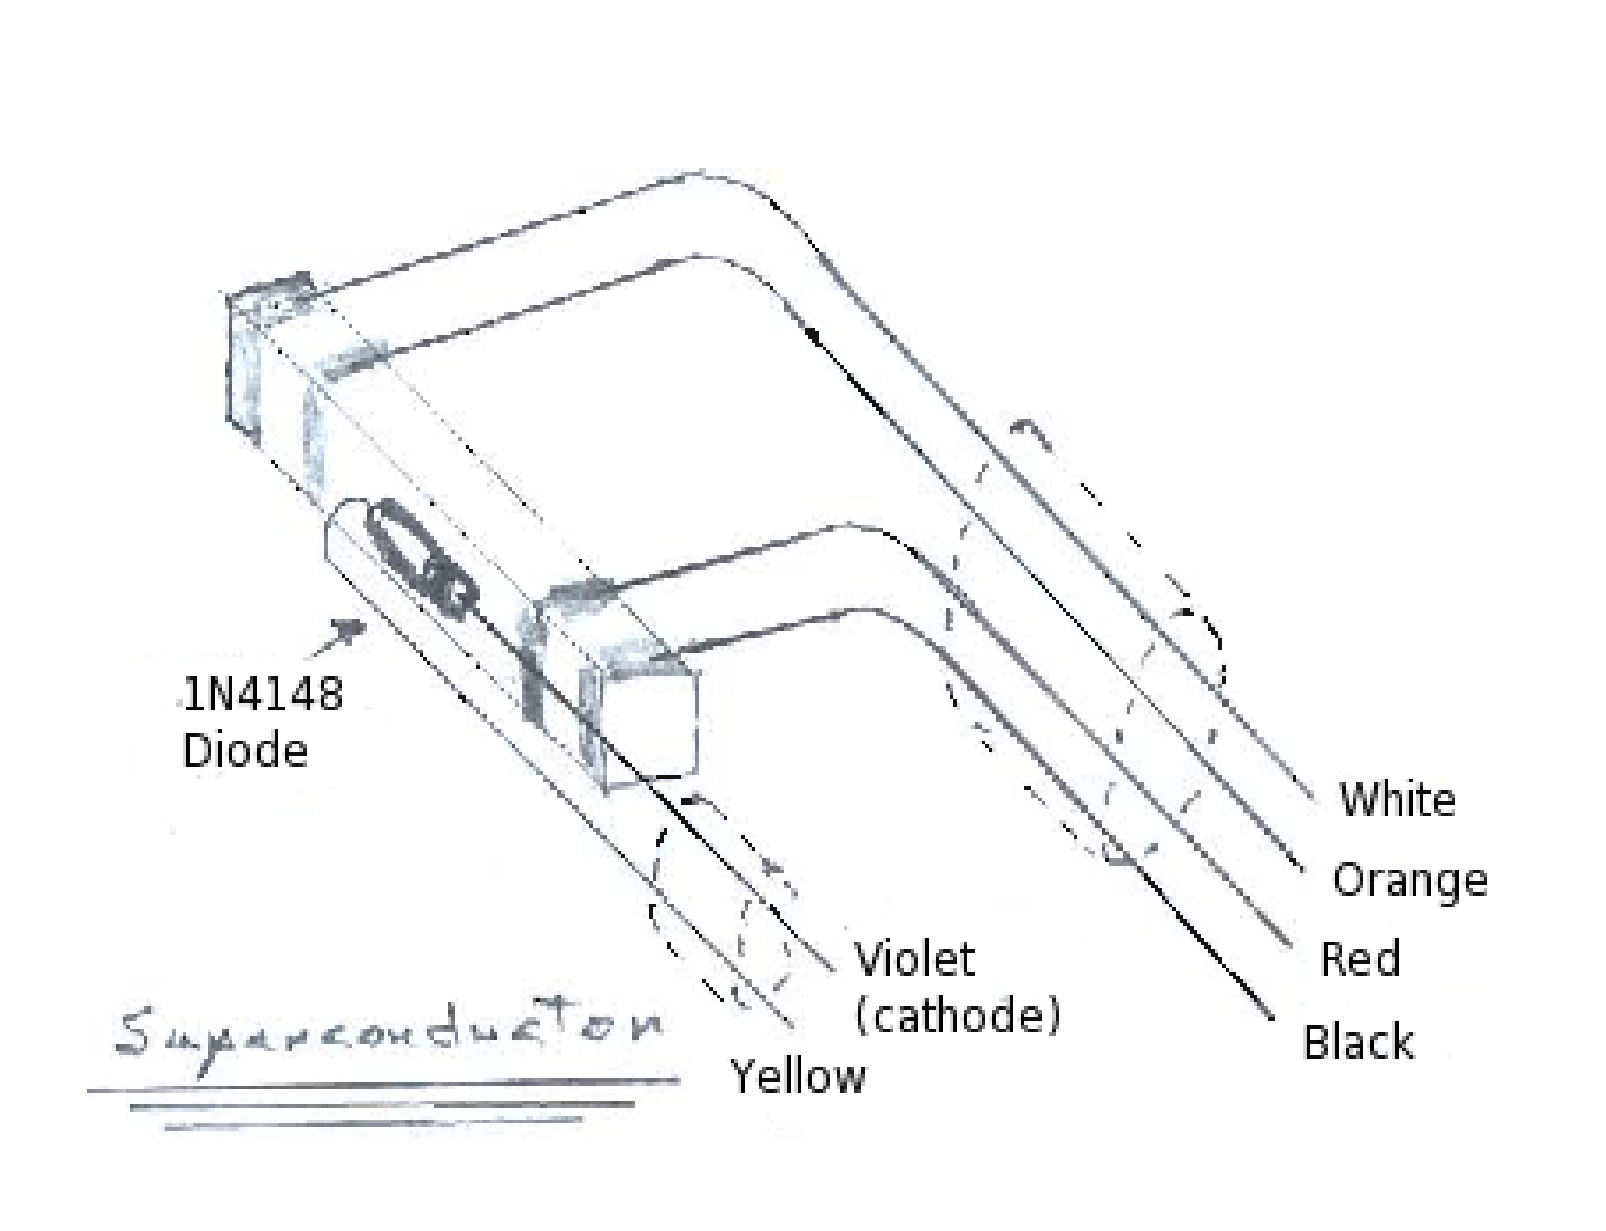
\includegraphics[width=\textwidth]{Figures/SuperconductorDrawing.eps}
                        \caption{Connection of superconductor and diode}
                        \label{fig:scDiode}
                  \end{minipage}
                  \hspace{0.5cm}
                  \begin{minipage}[b]{0.45\linewidth}
                        \centering
                        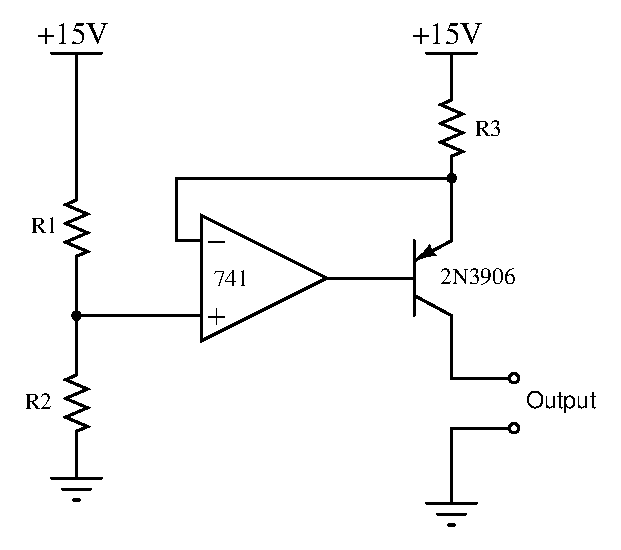
\includegraphics[width=\textwidth]{Figures/ConstantCurrent.eps}
                        \caption{Constant current supply circuit diagram}
                        \label{fig:constantCurrent}
                  \end{minipage}
            \end{figure}

            Another important part of the preparation phase was to calibrate the diode. The first step in this calibration process was to create a constant current supply. We did this by building a circuit like the one in \textbf{Figure} ~\ref{fig:constantCurrent}. In that circuit we used the following values: $R_1 = 1 \text{ k} \Omega$, $R_2 = 807 \text{ }\Omega$, and $R_3 = 820 \text{ \text{ k}} \Omega$. Using those resistor values produced a constant current of $10.3 \text{ }\mu A$. I then put the diode and a thermocouple in an ice bath and liquid nitrogen (LN) bath with $T_{ice} = 273.35$ K and $T_{LN} = 77.15$ K, respectively. the resultant voltages were $V_{ice} = 0.4595$ V and $V_{LN} = 0.9889$ V. I was then able to fit this data to a linear model of the form $V = V_0 + m T$, with $V_0 = 0.460024$ and $m = -0.002698$ (because there were only two data points, the fit was perfect).

             In order to measure the resistivity of the BSCCO superconductor, I needed to build a second constant current supply to run through the superconductor. I used the same circuit layout (see \textbf{Figure} ~\ref{fig:constantCurrent}), but this time with $R_1 = 952 \text{ }\Omega$, $R_2 = 332 \text{ } \Omega$, and $R_3 = 551 \text{ } \Omega$. The measured current output from this circuit was $20.17$ mA.

             The final step in the preparation phase was to build a LabVIEW VI that would measure the voltage drop across the diode (for temperature data) while simultaneously measuring the voltage drop across the superconductor (for resistivity). There were a few subtleties associated with this process. Because the resistivity is effectively zero while the BSCCO is superconducting, we needed to make sure the scale on the input for that voltage reading was very small. Also, because I was measuring two voltages at the same time, I needed to be sure that the measurements I was taking were actually the voltages across the diode and superconductor, and not the interaction between the two sources and the A/D converter. To do this I simply set the NI DAQ to sample the channel for each source 3 times and then I only looked at the last reading. This allowed the voltages to fully settle to their true values. The final minor step in building the VI was making sure that when we were reading the superconductor voltage (very small) we weren't getting poor data because of the intrinsic offset voltage of the DAQ. To do this we cooled the superconductor to LN temperatures and measured the voltage drop across the superconductor. Theoretically, this should be zero because at those temperatures we have supercontuctance, but we measured an offset voltage of $V_{offset} = -0.366 $ mV. To account for this we simply had to subtract $V_{offset}$ from all of our voltage readings for the superconductor.

      \subsection{Collection}

            Once the preparation phase was finished, we were ready to take the measurements. To take the measurements I set the system up by connecting the diode and superconductor to their respective constant current supplies, connecting each of them to the NI DAQ, and connecting the diode/superconductor to the inside of the cytrostat. I then took data in two phases: a quick scan of the temperature range from $80$ K to $280$ K, and a slow scan of the range from $80$ K to $130$ K. To do the quick scan I cooled the cyrostat to LN temperatures. After removing the system from the liquid nitrogen, I placed it on the table and used the VI to measure the data as it heated up to room temperature. Doing this quick sweep allowed me to get a pretty good idea about where the critical temperature was for my superconductor (see \textbf{Figure} ~\ref{fig:fastHeat}). To do the slow scan I started by cooling the system to LN temperature again. I then laid the cyrostat horizontally on the styrofoam LN container and placed another styrofoam container on top of that to hold in the fumes so the heater block wouldn't heat too quickly.



  \section{Results and Discussion}

      The results of my experiment match the reported data from the papers cited previously. As can been seen in \textbf{Figure} ~\ref{fig:fastHeat}\footnote{Here I would like to take time to thank Chuck for hard work making these figures look good}, my superconductor is still at zero resistance until about $T_c = 105.5$ K.  All of the values reported by other groups were in the range of $105-112$ K. The wide range of values could be due to a difference in how the transition temperature is defined. Looking at the plot for the slower scan in \textbf{Figure} ~\ref{fig:slowHeat} , the superconductor leaves the zero resistance state at about $105.5$ K, but it doesn't reach a stable value until about $111.5$ K. The fact that my value is lower than the average from the other papers could be a result of how $T_c$ was defined.

      \begin{figure}[h]
      \begin{minipage}[b]{0.48\linewidth}
      \begin{center}
            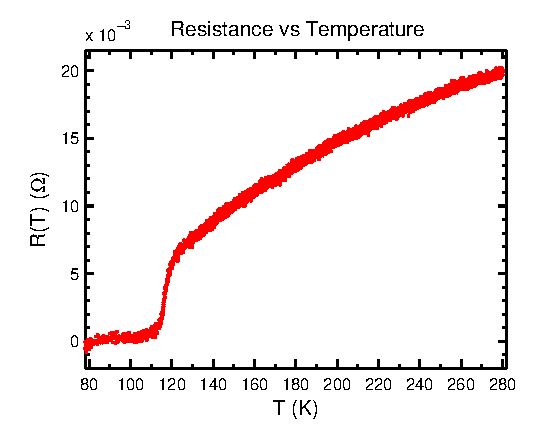
\includegraphics[width=\textwidth]{Figures/fastHeat2.eps}
            \caption{Heating data from quick scan of temperatures from $80 - 280$ K}
            \label{fig:fastHeat}
      \end{center}
      \end{minipage}
      \hspace{0.5cm}
      \begin{minipage}[b]{0.48\linewidth}
      \begin{center}
            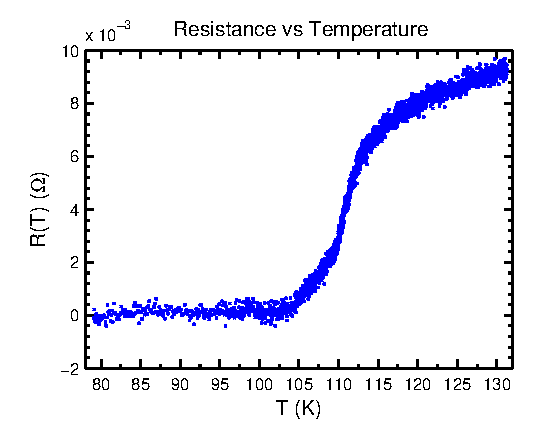
\includegraphics[width=\textwidth]{Figures/slowHeat2.eps}
            \caption{Heating data collected on slow scan of temperatures from $80 - 130$ K}
            \label{fig:slowHeat}
      \end{center}
      \end{minipage}
\end{figure}

      My superconductor had a near step-like behavior at $T_c$. Theory suggests that the transition should be a perfect step, so the fact that mine is very close is good. One explanation for why my transition is a little rounded could that the rate of temperature change was not constant. This matters because I read data at a constant rate of $100$ Hz, and trying to read non-constant rates using a constant sampling frequency can introduce error. Another explanation for the discrepancy in my curve is that the DAQ may not have been able to resolve such fast changes in the resistance.

      Another interesting property that is highlighted in the quick scan curve in \textbf{Figure} ~\ref{fig:fastHeat} is the behavior of the superconductor after it finishes the transition. In general, a standard metal will increase in resistivity as temperature increases and a standard semiconductor will decrease resistivity with an increase in temperature. The quick scan curve clearly shows that as temperature continues to increase beyond $T_c$, the resistivity of the material also increases, mimicking the behavior of of a metal.


  \clearpage
  \pagestyle{empty}
  \bibliography{scReport}

  %%% End document

\end{document}
